\documentclass[paper=a4, fontsize=11pt]{scrartcl}
\usepackage[T1]{fontenc}
\usepackage[utf8]{inputenc}
\usepackage{lmodern}
\usepackage{multirow}
\usepackage[table,xcdraw]{xcolor}
\usepackage[spanish]{babel}
\usepackage{cite}
\usepackage{amsmath,amsfonts,amsthm} % Math packages
\usepackage{graphics,graphicx, float} %para incluir imágenes y colocarlas
\usepackage[backref,colorlinks=true,linkcolor=black,urlcolor=blue,citecolor=blue]{hyperref} %Para crear enlaces en el pdf
\usepackage{url}
\usepackage[shortlabels]{enumitem}
\usepackage{appendix}
\usepackage{eurosym}
\usepackage{epsfig}
\usepackage{caption}
\usepackage{subcaption}

\usepackage{xcolor}
\usepackage{framed}
\definecolor{shadecolor}{RGB}{239, 251, 255}

\usepackage{listings}
\usepackage{color}

\definecolor{dkgreen}{rgb}{0,0.6,0}
\definecolor{gray}{rgb}{0.5,0.5,0.5}
\definecolor{mauve}{rgb}{0.58,0,0.82}
\definecolor{lgrey}{rgb}{0.9,0.9,0.9}


\lstset{frame=tb,
  language=C++,
  aboveskip=3mm,
  belowskip=3mm,
  showstringspaces=false,
  columns=flexible,
  basicstyle={\small\ttfamily},
  numbers=none,
  numberstyle=\tiny\color{gray},
  keywordstyle=\color{blue},
  commentstyle=\color{dkgreen},
  stringstyle=\color{mauve},
  breaklines=true,
  breakatwhitespace=true,
  tabsize=3
}

\renewcommand{\appendixname}{Anexo}
\renewcommand{\appendixtocname}{Anexo}
\renewcommand{\appendixpagename}{Anexo}

\numberwithin{figure}{section} % Number figures within sections (i.e. 1.1, 1.2, 2.1, 2.2 instead of 1, 2, 3, 4)
\numberwithin{table}{section} % Number tables within sections (i.e. 1.1, 1.2, 2.1, 2.2 instead of 1, 2, 3, 4)
\newcommand{\horrule}[1]{\rule{\linewidth}{#1}} % Create horizontal rule command with 1 argument of height

\title{
    \normalfont \normalsize
    \textsc{{\textbf{Algorítmica (2016-2017)}} \\ Grado en Ingeniería Informática \\ Universidad de Granada} \\ [25pt] % Your university, school and/or department name(s)
    \horrule{0.5pt} \\[0.4cm] % Thin top horizontal rule
    \huge Memoria Práctica 4: Backtracking y Branch & Bound\\ % The assignment title
    \horrule{2pt} \\[0.5cm] % Thick bottom horizontal rule
}
\author{Antonio de la Vega Jiménez }

%*************************************************************


\begin{document}

\maketitle % Muestra el Título
\newpage %inserta un salto de página
\tableofcontents % para generar el índice de contenidos
\listoffigures
\newpage

%*************************************************************

\section{Información PC usado}

\subsection{Hardware}
El hardware usado tiene las siguientes características:
\begin{itemize}
  \item \textbf{CPU:} \texttt{Intel(R) Core(TM) i3 CPU 540}
  \item \textbf{Velocidad reloj:} \texttt{3.07GHz}
  \item \textbf{Caché:} \texttt{4096 KB}
  \item \textbf{RAM:} \texttt{6039668 kB  }
\end{itemize}
\subsection{Software}
\subsubsection{Sistema operativo}
\begin{itemize}
  \item \textbf{SO:} \texttt{Manjaro Linux}
  \item \textbf{Kernel:}\texttt{ 4.9.30-1-MANJARO}
\end{itemize}
\subsubsection{Compilador}
\begin{itemize}
  \item \textbf{Versión compilador:} \texttt{g++ (GCC) 7.1.1 20170528}
\end{itemize}




\section{Descripción del problema}
La empresa Friendship se ocupa de encontrar amistades formadas entre dos personas. Con
tal objetivo tenemos un conjunto de personas (con número par de personas) y tenemos que
encontrar las parejas de amigos que minimicen la discrepancia global. 

Con esta información de gustos por cada individuo podemos obtener una matriz de
discrepancias entre individuos siendo calculada como:
\begin{equation}
    D(i,h) = \sum_{k=1}^{ncar}|M (i,k)- M (j , k )| \quad \forall i\neq j \quad D(i,j)= \infty \quad si \quad i= j
\end{equation}

Nuestro objetivo es obtener las mejores parejas de individuos que minimicen la discrepancia
total. Así una solución cumple que :


\begin{equation}
    minimiza \quad D(i,h) = \sum_{i=1}^{npersonas}D(i , X(i))
\end{equation}


\section{Solución con voraces}

El código usado es el mostrado a continuación

\begin{lstlisting}
vector <pair<int, int>> asignParejas(vector <vector<int>> matriz) {
    vector <pair<int, int>> sol;
    vector<int> selec;

    int max = numeric_limits<int>::max();
    int per1, per2, min;

    for (per1 = 0; per1 < matriz.size(); ++per1) {
        min = max;

        if (!contains(selec, per1)) {
            for (int j = 0; j < matriz[per1].size(); ++j) {
                if (matriz[per1][j] < min && !contains(selec, j)) {
                    min = matriz[per1][j];
                    per2 = j;
                }
            }
        } else {
            per2 = buscarPareja(per1, sol);
        }

        selec.push_back(per1);
        selec.push_back(per2);
        sol.push_back(make_pair(per1, per2));
    }

    return sol;
}
\end{lstlisting}

\subsection{Eficiencia teórica}
Suponiendo que la función contains tiene una eficiencia constante, nuestro algoritmo tendrá que recorrer la matriz, y la eficiencia será:
  \begin{equation}
      O(n^2)
  \end{equation}

\subsection{Eficiencia empírica}

Al representar los datos obtenemos la siguiente gráfica:

\begin{figure}[H]
    \begin{center}
        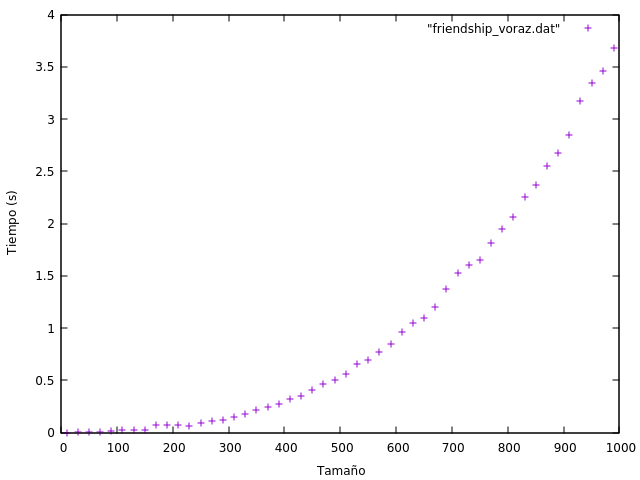
\includegraphics[scale=0.7]{imagenes/voraz.png}
        \caption{Tiempos de ejecución.}
        \label{fig2}
    \end{center}
\end{figure}

\subsection{Ajuste curva teórica a empírica}

En este paso realizamos el siguiente ajuste:
\begin{shaded*}
\begin{verbatim}
gnuplot> f(x) = a*x*x + b*x + c
gnuplot> fit f(x) "friendship_voraz.dat" via a,b,c
\end{verbatim}
\end{shaded*}

De forma que obtenemos los siguientes parámetros:

\begin{shaded*}
\begin{verbatim}
Final set of parameters            Asymptotic Standard Error
=======================            ==========================
a               = 5.42881e-06      +/- 1.304e-07    (2.402%)
b               = -0.00196063      +/- 0.0001347    (6.87%)
c               = 0.170102         +/- 0.02916      (17.14%)
\end{verbatim}
\end{shaded*}

Y finalmente obtenemos la siguiente función ajustada:
\begin{figure}[H]
    \begin{center}
        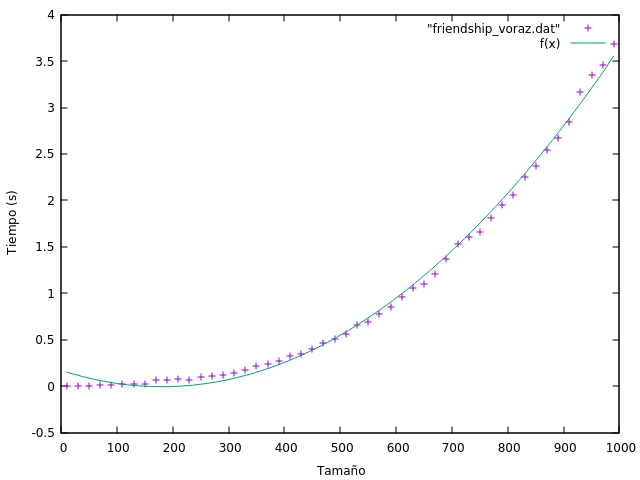
\includegraphics[scale=0.7]{imagenes/vorazadj.png}
        \caption{Ajuste eficiencia teórica y empírica.}
        \label{fig3}
    \end{center}
\end{figure}

%*************************************
%*************************************
%*************************************
%*************************************



\section{Solución Backtracking}

\subsection{Sin Poda}
El código usado es el mostrado a continuación

\begin{lstlisting}
int asignParejas(int n, Apermutacion &ab, const vector <vector<int>> &D) {
    Apermutacion P(n);
    bool seguir = true;
    int bact = 0;
    int best_discrepancia = numeric_limits<int>::max();
    unsigned int nodos_recorridos = 0;
    while (seguir) {

        nodos_recorridos++;
        bact = Suma_Discrepancias(P, D);

        if (P.GetLevel() == n - 1) { //Hoja
            if (bact < best_discrepancia) {
                best_discrepancia = bact;
                ab = P;
                seguir = P.Backtracking();
            } else seguir = P.GeneraSiguienteProfundidad();
        } else seguir = P.GeneraSiguienteProfundidad();

    }
    return best_discrepancia;
}
\end{lstlisting}


\subsubsection{Eficiencia teórica}

La eficiencia depende del tamaño de la matriz, si tenemos n elementos y de el uso de un árbol permutacional:

  \begin{equation}
      \sum_{i=1}^{n} \dfrac{n!}{n - i!} \rightarrow O(n!)
  \end{equation}

\subsubsection{Eficiencia empírica}

Al representar los datos obtenemos la siguiente gráfica:

\begin{figure}[H]
    \begin{center}
        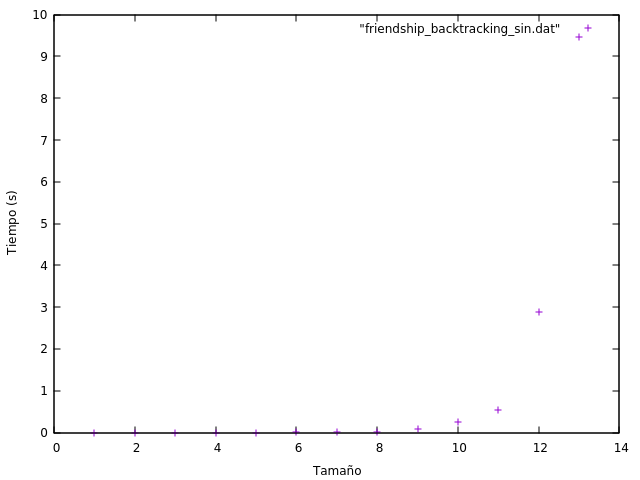
\includegraphics[scale=0.7]{imagenes/bts.png}
        \caption{Tiempos de ejecución.}
        \label{fig19}
    \end{center}
\end{figure}

\subsubsection{Ajuste curva teórica a empírica}

\begin{shaded*}
\begin{verbatim}
gnuplot> fac(x) = (int(x)==0) ? 1.0 : int(x) * fac(int(x)-1.0)
gnuplot> f(x) = a*x*fac(x)
gnuplot> fit f(x) "friendship_backtracking_sin.dat" via a
\end{verbatim}
\end{shaded*}

De forma que obtenemos los siguientes parámetros:

\begin{shaded*}
\begin{verbatim}
Final set of parameters            Asymptotic Standard Error
=======================            ==========================
a               = 1.18871e-10      +/- 8.09e-12     (6.805%)

\end{verbatim}
\end{shaded*}

Y finalmente obtenemos la siguiente función ajustada:
\begin{figure}[H]
    \begin{center}
        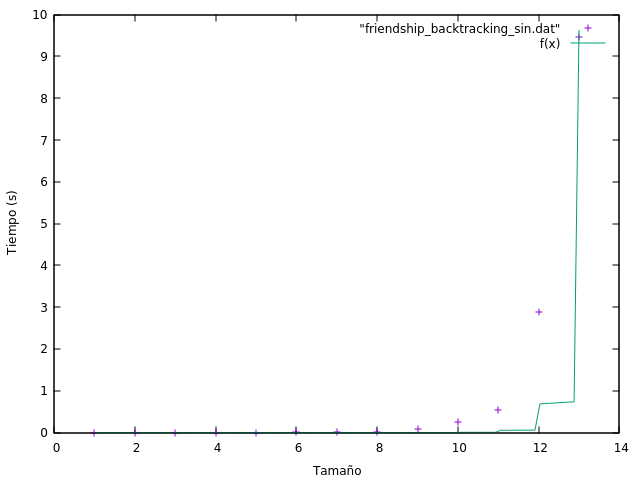
\includegraphics[scale=0.7]{imagenes/btsadj.png}
        \caption{Ajuste eficiencia teórica y empírica.}
        \label{fig20}
    \end{center}
\end{figure}



\subsection{Con Poda}
El código usado es el mostrado a continuación

\begin{lstlisting}
int asignParejas(int n, Apermutacion &ab, const vector <vector<int>> &D) {
    Apermutacion P(n);
    bool seguir = true;
    int bact = 0;
    int best_discrepancia = numeric_limits<int>::max();
    unsigned int nodos_recorridos = 0;
    while (seguir) {

        nodos_recorridos++;
        bact = Suma_Discrepancias(P, D);

        if (P.GetLevel() == n - 1) { //Hoja
            if (bact < best_discrepancia) {
                best_discrepancia = bact;
                ab = P;
                seguir = P.Backtracking();
            } else seguir = P.GeneraSiguienteProfundidad();
        } else {
            vector<vector<int>> no_asignados = obtenerNoAsignados(D,P);
            int mejor_estimado = calcularEstimacion(no_asignados);

            if(mejor_estimado + bact >= best_discrepancia) {
                seguir = P.Backtracking();
            } else {
                seguir = P.GeneraSiguienteProfundidad();
            }
        }
    }

    return best_discrepancia;
}
\end{lstlisting}


\subsubsection{Eficiencia teórica}

La eficiencia depende del tamaño de la matriz, si tenemos n elementos y de el uso de un árbol permutacional:

  \begin{equation}
      \sum_{i=1}^{n} \dfrac{n!}{n - i!} \rightarrow O(n!)
  \end{equation}

\subsubsection{Eficiencia empírica}

Al representar los datos obtenemos la siguiente gráfica:

\begin{figure}[H]
    \begin{center}
        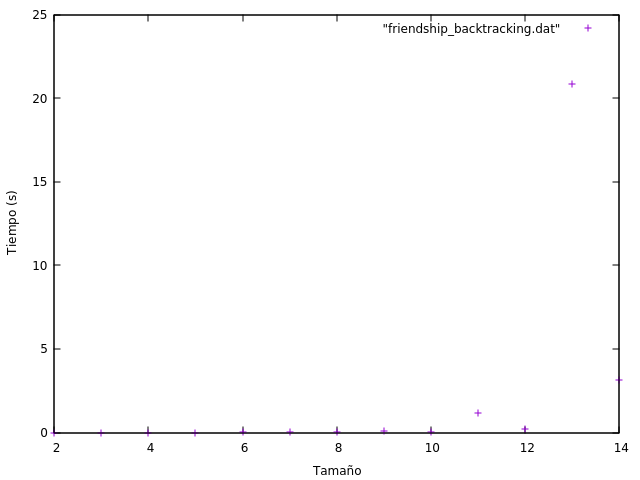
\includegraphics[scale=0.7]{imagenes/bt.png}
        \caption{Tiempos de ejecución.}
        \label{fig19}
    \end{center}
\end{figure}

\subsubsection{Ajuste curva teórica a empírica}

\begin{shaded*}
\begin{verbatim}
gnuplot> fac(x) = (int(x)==0) ? 1.0 : int(x) * fac(int(x)-1.0)
gnuplot> f(x) = a*x*fac(x)
gnuplot> fit f(x) "friendship_backtracking.dat" via a
\end{verbatim}
\end{shaded*}

De forma que obtenemos los siguientes parámetros:

\begin{shaded*}
\begin{verbatim}
Final set of parameters            Asymptotic Standard Error
=======================            ==========================
a               = 3.70117e-12      +/- 4.863e-12    (131.4%)
\end{verbatim}
\end{shaded*}

Y finalmente obtenemos la siguiente función ajustada:
\begin{figure}[H]
    \begin{center}
        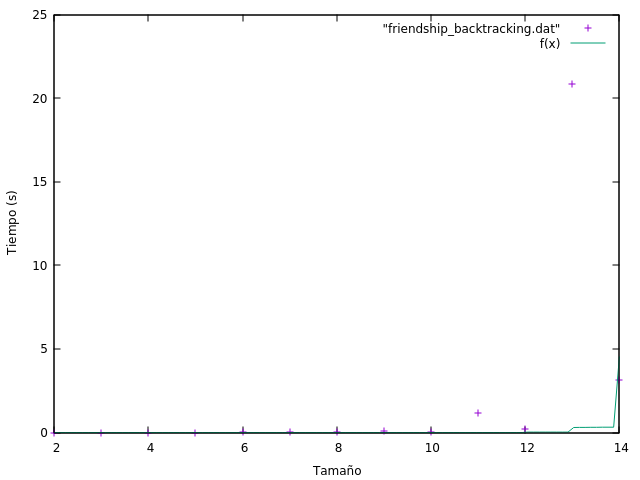
\includegraphics[scale=0.7]{imagenes/btadj.png}
        \caption{Ajuste eficiencia teórica y empírica.}
        \label{fig20}
    \end{center}
\end{figure}

%*************************************
%*************************************
%*************************************
%*************************************

\section{Solución Branch \& Bound}

\begin{itemize}
    \item \textbf{Cálculo de cotas:}
    \begin{itemize}
        \item \textit{Cota inferior (CI):} Como cota inferior usaremos una estrategia greedy, sin la restricción de que no se pueden repetir parejas, por lo cual obtendremos la mínima discrepancia posible.
        \item \textit{Cota Superior (CS):} Como cota superior usaremos una estrategia greedy cumpliendo la restricción de que no se pueden repetir parejas.
    \end{itemize}
\end{itemize}

Para realizar la poda comprobamos si lo mejor que podemos obtener ( CI ), es peor que nuestra CS o que la mejor solución de las que hemos encontrado.\newline



El código usado es el mostrado a continuación

\begin{lstlisting}
int asignParejas(int n, Apermutacion &ab, const vector <vector<int>> &D) {
    Apermutacion P(n);

    int dactual = 0;
    int best_discrepancia = numeric_limits<int>::max();

    vector<int> aux;
    vector<int> asignados(0);

    int CI = cotaInferior(D,asignados);
    int CS = cotaSuperior(D,asignados);
    int C = CS;
    int DE = (CI+CS)/2;

    int nodos_recorridos = 0;
    priority_queue<nodo> pq;

    nodo a(dactual,CI,DE,CS,P);
    pq.push(a);

    do {
        nodos_recorridos++;
        nodo a = pq.top();  pq.pop();

        vector<vector<int> > hijos = a.ab.GeneraHijos();

        for (int i=0; i< (int)hijos.size(); i++) {

            Apermutacion H (hijos[i],a.ab.GetLevel()+1);

            dactual=Suma_Discrepancias(H,D);
            aux = obtenerAsignaciones(H);

            CI= dactual+cotaInferior(D,aux);
            CS= dactual+cotaSuperior(D,aux);
            DE= (CS+CI)/2;

            if (H.GetLevel()==n-1 && dactual<best_discrepancia) {
                ab=H;
                best_discrepancia=dactual;
                C=(C>dactual)?dactual: C;
            } else {
                if (CI<=C ) {
                    nodo anew (dactual,CI,DE,CS,H);
                    pq.push(anew);
                    C= (C>CS)? CS:C;
                }
            }
        }

    } while (!pq.empty());


    return best_discrepancia;
}
\end{lstlisting}

\subsection{Eficiencia teórica}

Al tener un árbol Permutacionalpodemos llegar a generar:
 
  \begin{equation}
      \sum_{i=1}^{n} \prod_{j = n-(i-1)}^{n} j \rightarrow O(n*n!)
  \end{equation}

 
\subsection{Eficiencia empírica}

Al representar los datos obtenemos la siguiente gráfica:

\begin{figure}[H]
    \begin{center}
        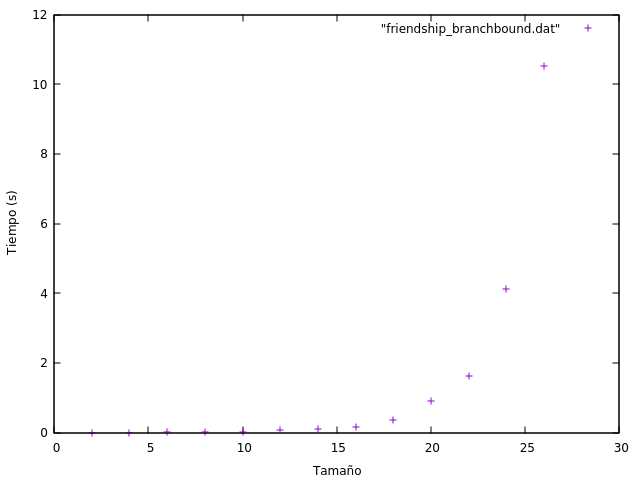
\includegraphics[scale=0.7]{imagenes/bb.png}
        \caption{Tiempos de ejecución.}
        \label{fig2}
    \end{center}
\end{figure}

\subsection{Ajuste curva teórica a empírica}

En este paso realizamos el siguiente ajuste:
\begin{shaded*}
\begin{verbatim}
gnuplot> fac(x) = (int(x)==0) ? 1.0 : int(x) * fac(int(x)-1.0)
gnuplot> f(x) = a*x*fac(x)
gnuplot> fit f(x) "friendship_branchbound.dat" via a

\end{verbatim}
\end{shaded*}

De forma que obtenemos los siguientes parámetros:

\begin{shaded*}
\begin{verbatim}
Final set of parameters            Asymptotic Standard Error
=======================            ==========================
a               = 3.70117e-12      +/- 4.863e-12    (131.4%)
\end{verbatim}
\end{shaded*}

Y finalmente obtenemos la siguiente función ajustada:
\begin{figure}[H]
    \begin{center}
        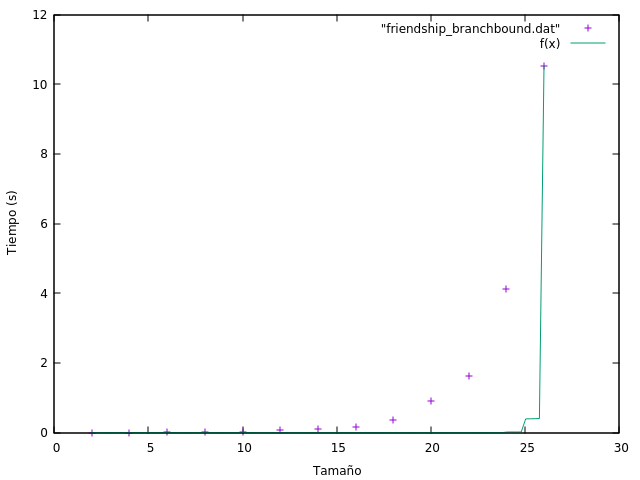
\includegraphics[scale=0.7]{imagenes/bbadj.png}
        \caption{Ajuste eficiencia teórica y empírica.}
        \label{fig3}
    \end{center}
\end{figure}
%*************************************************************

\section{Comparativa Bactracking y Branch \& Bound }

Debido a la gran diferencia de nodos explorados, he mostrado los resultados en una tabla, ya que en una gráfica no se veían con claridad.

\begin{table}[H]
\centering
\label{my-label}
\begin{tabular}{|
>{\columncolor[HTML]{EFEFEF}}c |c|c|c|}
\hline
\multicolumn{1}{|l|}{\cellcolor[HTML]{EFEFEF}\textit{Tamaño}} & \multicolumn{1}{l|}{\cellcolor[HTML]{EFEFEF}Bactracking sin poda} & \multicolumn{1}{l|}{\cellcolor[HTML]{EFEFEF}Backtracking con poda} & \multicolumn{1}{l|}{\cellcolor[HTML]{EFEFEF}Branch \& Bound} \\ \hline
2 & \textit{\textbf{3}} & \textit{\textbf{3}} & \textit{\textbf{2}} \\ \hline
4 & \textit{\textbf{13}} & \textit{\textbf{10}} & \textit{\textbf{4}} \\ \hline
6 & \textit{\textbf{76}} & \textit{\textbf{48}} & \textit{\textbf{8}} \\ \hline
8 & \textit{\textbf{633}} & \textit{\textbf{238}} & \textit{\textbf{13}} \\ \hline
10 & \textit{\textbf{6331}} & \textit{\textbf{926}} & \textit{\textbf{19}} \\ \hline
12 & \textit{\textbf{75973}} & \textit{\textbf{3247}} & \textit{\textbf{43}} \\ \hline
\end{tabular}
\caption{Nodos explorados}

\end{table}

\newpage

\end{document}
